% =====================================================================
% Research Methodology Architecture Diagram (Phase 2, Revision 3) -- decision horizons
% Standalone TikZ source. Compile with:  pdflatex methodology_architecture.tex
% The resulting methodology_architecture.pdf is included by cn_phase2.tex.
% Every box is labelled with the methodology step (Section 10) it implements.
% =====================================================================
\documentclass[tikz,border=4pt]{standalone}
\usepackage[T1]{fontenc}
\usepackage{lmodern}
\usepackage{amsmath,amssymb}
\usetikzlibrary{arrows.meta,positioning,calc,fit,backgrounds}
\renewcommand{\familydefault}{\sfdefault}

\definecolor{cData}{HTML}{2B6CB0}
\definecolor{cPrep}{HTML}{4A5568}
\definecolor{cModel}{HTML}{C05621}
\definecolor{cBase}{HTML}{2F855A}
\definecolor{cExp}{HTML}{6B46C1}
\definecolor{cEval}{HTML}{B7791F}
\definecolor{cOut}{HTML}{1A202C}

\tikzset{
  box/.style={draw=#1, fill=#1!9, rounded corners=2.5pt, line width=0.7pt,
              align=center, font=\sffamily\footnotesize, inner sep=3pt,
              text=black},
  hdr/.style={font=\sffamily\bfseries\footnotesize, text=#1},
  arr/.style={-{Stealth[length=2.4mm,width=1.8mm]}, line width=0.75pt, draw=black!65},
  darr/.style={arr, dashed},
  band/.style={draw=black!35, dashed, rounded corners=4pt, line width=0.5pt},
  bandlbl/.style={font=\sffamily\bfseries\scriptsize, text=black!60, anchor=north west,
                  fill=white, inner sep=1.5pt},
  lbl/.style={font=\sffamily\scriptsize, text=black!75}
}
% Band titles are drawn on a foreground layer so that arrows pass beneath them.
\pgfdeclarelayer{foreground}
\pgfsetlayers{main,foreground}

\begin{document}
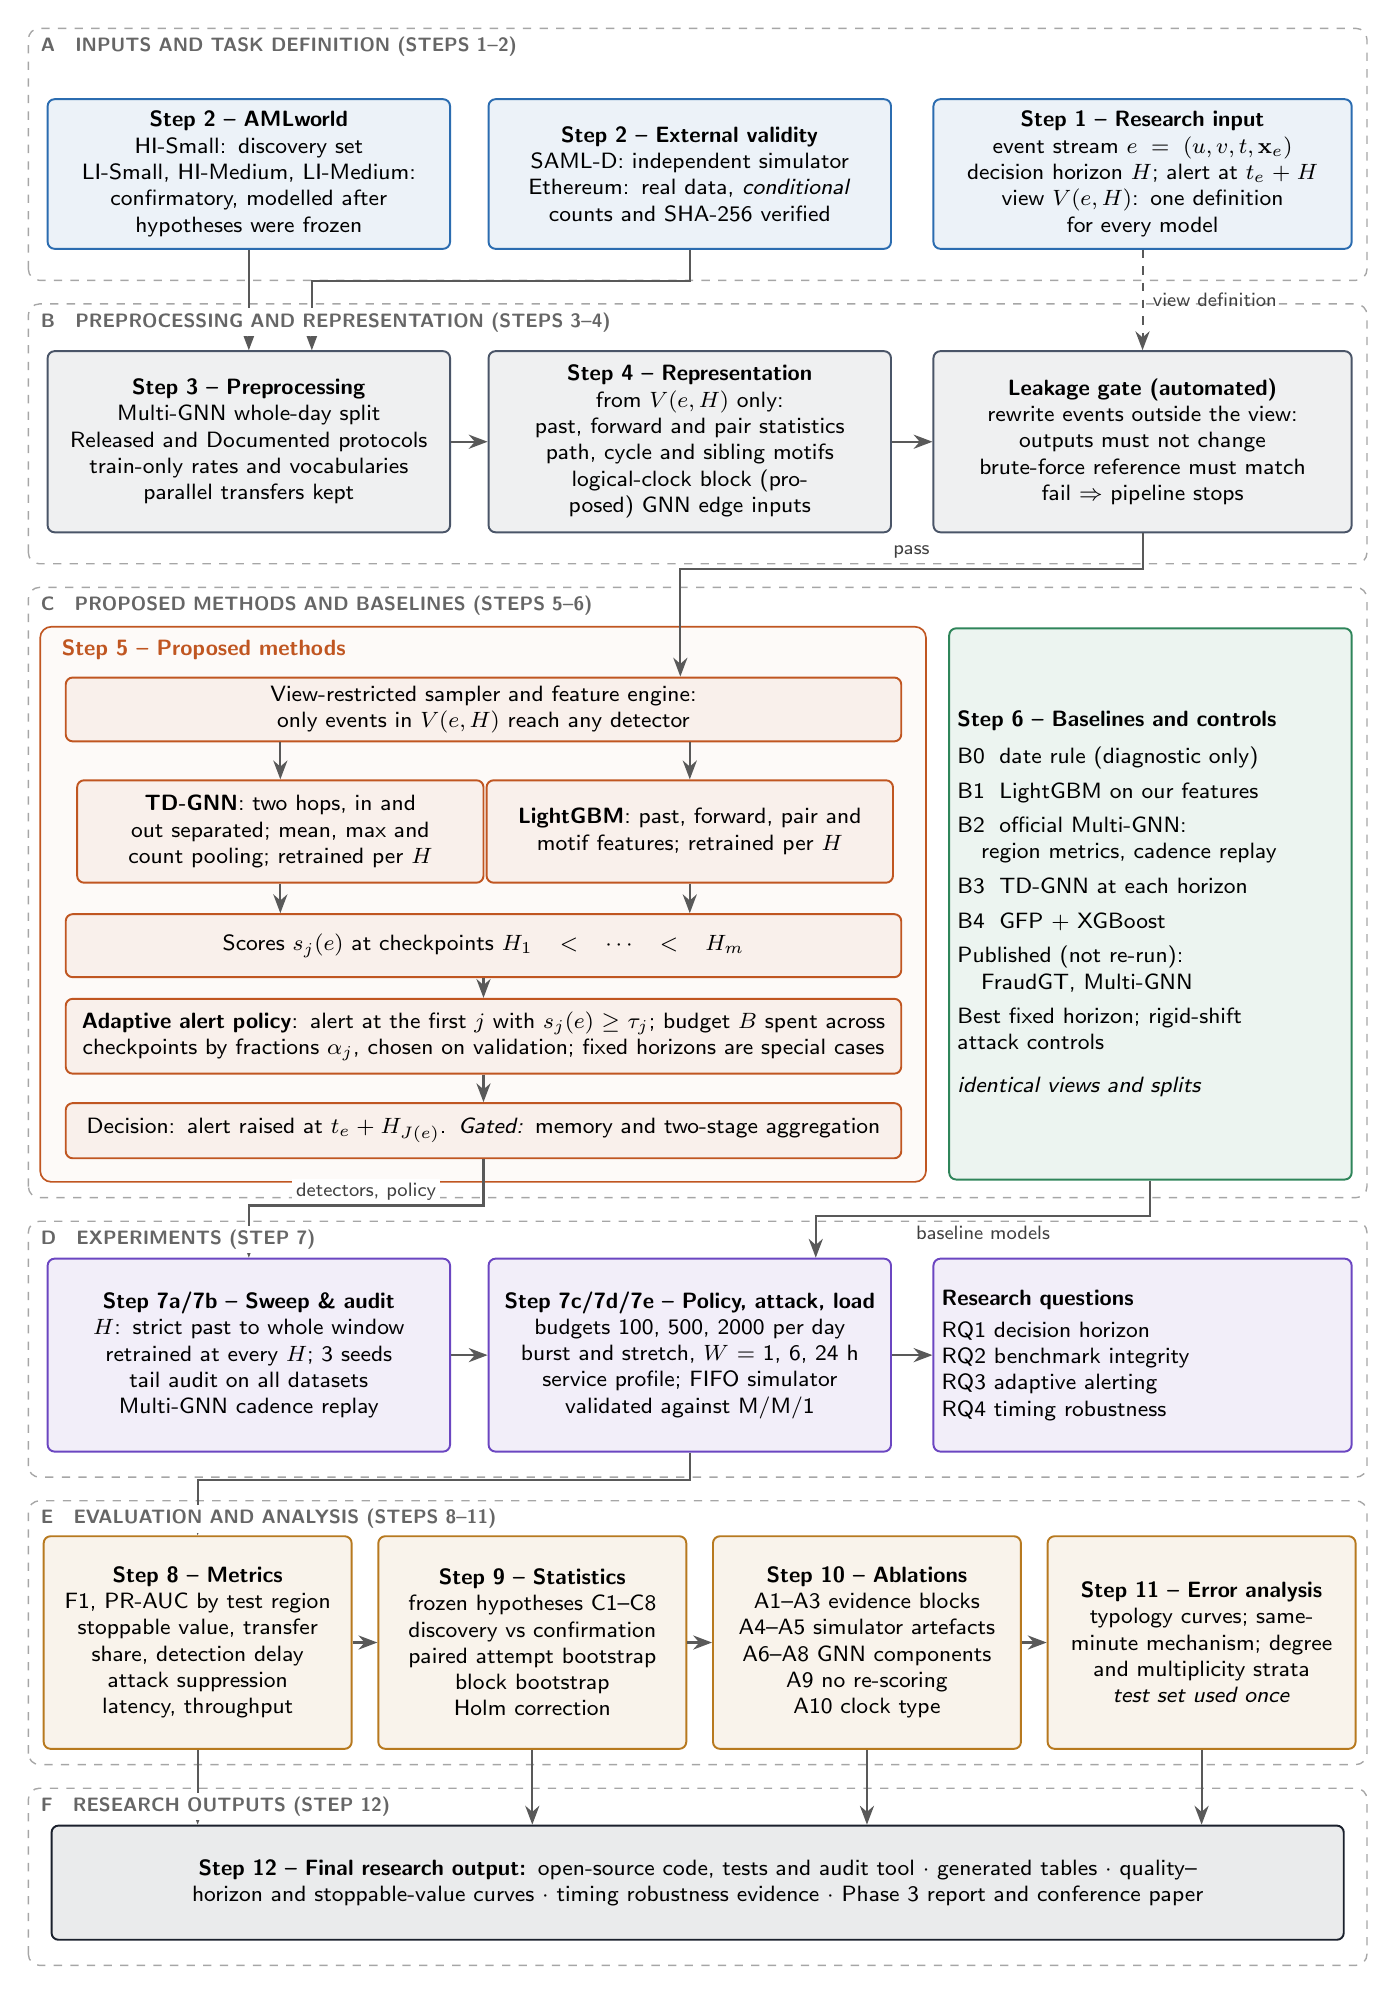
\begin{tikzpicture}[x=1cm,y=1cm]

% ------------------------------------------------------------- bands
\draw[band] (0,21.4) rectangle (17.0,24.6);
\draw[band] (0,17.8) rectangle (17.0,21.1);
\draw[band] (0,9.75) rectangle (17.0,17.5);
\draw[band] (0,6.2) rectangle (17.0,9.45);
\draw[band] (0,2.55) rectangle (17.0,5.9);
\draw[band] (0,0.0) rectangle (17.0,2.25);
\begin{pgfonlayer}{foreground}
\node[bandlbl] at (0.1,24.55) {A \; INPUTS AND TASK DEFINITION (STEPS 1--2)};
\node[bandlbl] at (0.1,21.05) {B \; PREPROCESSING AND REPRESENTATION (STEPS 3--4)};
\node[bandlbl] at (0.1,17.45) {C \; PROPOSED METHODS AND BASELINES (STEPS 5--6)};
\node[bandlbl] at (0.1,9.4) {D \; EXPERIMENTS (STEP 7)};
\node[bandlbl] at (0.1,5.85) {E \; EVALUATION AND ANALYSIS (STEPS 8--11)};
\node[bandlbl] at (0.1,2.2) {F \; RESEARCH OUTPUTS (STEP 12)};
\end{pgfonlayer}

% ------------------------------------------------------------- band A
\node[box=cData, text width=4.9cm, minimum height=1.9cm] (d1) at (2.8,22.75)
  {\textbf{Step 2 -- AMLworld}\\ HI-Small: discovery set\\ LI-Small, HI-Medium, LI-Medium:\\ confirmatory, modelled after\\ hypotheses were frozen};
\node[box=cData, text width=4.9cm, minimum height=1.9cm] (d2) at (8.4,22.75)
  {\textbf{Step 2 -- External validity}\\ SAML-D: independent simulator\\ Ethereum: real data, \emph{conditional}\\ counts and SHA-256 verified};
\node[box=cData, text width=5.1cm, minimum height=1.9cm] (task) at (14.15,22.75)
  {\textbf{Step 1 -- Research input}\\ event stream $e=(u,v,t,\mathbf{x}_e)$\\ decision horizon $H$; alert at $t_e+H$\\ view $V(e,H)$: one definition\\ for every model};

% ------------------------------------------------------------- band B
\node[box=cPrep, text width=4.9cm, minimum height=2.3cm] (prep) at (2.8,19.35)
  {\textbf{Step 3 -- Preprocessing}\\ Multi-GNN whole-day split\\ Released and Documented protocols\\ train-only rates and vocabularies\\ parallel transfers kept};
\node[box=cPrep, text width=4.9cm, minimum height=2.3cm] (repr) at (8.4,19.35)
  {\textbf{Step 4 -- Representation}\\ from $V(e,H)$ only:\\ past, forward and pair statistics\\ path, cycle and sibling motifs\\ logical-clock block (proposed)\ GNN edge inputs};
\node[box=cPrep, text width=5.1cm, minimum height=2.3cm] (gate) at (14.15,19.35)
  {\textbf{Leakage gate (automated)}\\ rewrite events outside the view:\\ outputs must not change\\ brute-force reference must match\\ fail $\Rightarrow$ pipeline stops};

% ------------------------------------------------------------- band C (methods)
\draw[draw=cModel, rounded corners=4pt, line width=0.6pt, fill=cModel!3] (0.15,9.95) rectangle (11.4,17.0);
\node[hdr=cModel, anchor=west] at (0.3,16.7) {Step 5 -- Proposed methods};
\node[box=cModel, text width=10.4cm, minimum height=0.8cm] (samp) at (5.78,15.95)
  {View-restricted sampler and feature engine: only events in $V(e,H)$ reach any detector};
\node[box=cModel, text width=4.95cm, minimum height=1.3cm] (gnn) at (3.2,14.4)
  {\textbf{TD-GNN}: two hops, in and out separated; mean, max and count pooling; retrained per $H$};
\node[box=cModel, text width=4.95cm, minimum height=1.3cm] (gbt) at (8.4,14.4)
  {\textbf{LightGBM}: past, forward, pair and motif features; retrained per $H$};
\node[box=cModel, text width=10.4cm, minimum height=0.8cm] (scr) at (5.78,12.95)
  {Scores $s_j(e)$ at checkpoints $H_1<\dots<H_m$};
\node[box=cModel, text width=10.4cm, minimum height=0.95cm] (pol) at (5.78,11.8)
  {\textbf{Adaptive alert policy}: alert at the first $j$ with $s_j(e)\ge\tau_j$; budget $B$ spent across\\ checkpoints by fractions $\alpha_j$, chosen on validation; fixed horizons are special cases};
\node[box=cModel, text width=10.4cm, minimum height=0.7cm] (head) at (5.78,10.6)
  {Decision: alert raised at $t_e+H_{J(e)}$. \emph{Gated:} memory and two-stage aggregation};

\draw[arr] (samp.south -| gnn) -- (gnn.north);
\draw[arr] (samp.south -| gbt) -- (gbt.north);
\draw[arr] (gnn.south) -- (gnn.south |- scr.north);
\draw[arr] (gbt.south) -- (gbt.south |- scr.north);
\draw[arr] (scr) -- (pol);
\draw[arr] (pol) -- (head);

% ------------------------------------------------------------- band C (baselines)
\node[box=cBase, text width=4.9cm, minimum height=7.0cm, align=left] (base) at (14.25,13.48)
  {\textbf{Step 6 -- Baselines and controls}\\[4pt]
   B0\; date rule (diagnostic only)\\[3pt]
   B1\; LightGBM on our features\\[3pt]
   B2\; official Multi-GNN:\\ \quad region metrics, cadence replay\\[3pt]
   B3\; TD-GNN at each horizon\\[3pt]
   B4\; GFP + XGBoost\\[3pt]
   Published (not re-run):\\ \quad FraudGT, Multi-GNN\\[3pt]
   Best fixed horizon; rigid-shift\\ attack controls\\[6pt]
   \textit{identical views and splits}};

% ------------------------------------------------------------- band D
\node[box=cExp, text width=4.9cm, minimum height=2.45cm] (train) at (2.8,7.75)
  {\textbf{Step 7a/7b -- Sweep \& audit}\\ $H$: strict past to whole window\\ retrained at every $H$; 3 seeds\\ tail audit on all datasets\\ Multi-GNN cadence replay};
\node[box=cExp, text width=4.9cm, minimum height=2.45cm] (harn) at (8.4,7.75)
  {\textbf{Step 7c/7d/7e -- Policy, attack, load}\\ budgets 100, 500, 2000 per day\\ burst and stretch, $W$ = 1, 6, 24 h\\ service profile; FIFO simulator\\ validated against M/M/1};
\node[box=cExp, text width=5.1cm, minimum height=2.45cm, align=left] (rq) at (14.15,7.75)
  {\textbf{Research questions}\\[2pt]
   RQ1 decision horizon\\
   RQ2 benchmark integrity\\
   RQ3 adaptive alerting\\
   RQ4 timing robustness};

% ------------------------------------------------------------- band E
\node[box=cEval, text width=3.7cm, minimum height=2.7cm] (met) at (2.15,4.1)
  {\textbf{Step 8 -- Metrics}\\ F1, PR-AUC by test region\\ stoppable value, transfer\\ share, detection delay\\ attack suppression\\ latency, throughput};
\node[box=cEval, text width=3.7cm, minimum height=2.7cm] (sta) at (6.4,4.1)
  {\textbf{Step 9 -- Statistics}\\ frozen hypotheses C1--C8\\ discovery vs confirmation\\ paired attempt bootstrap\\ block bootstrap\\ Holm correction};
\node[box=cEval, text width=3.7cm, minimum height=2.7cm] (abl) at (10.65,4.1)
  {\textbf{Step 10 -- Ablations}\\ A1--A3 evidence blocks\\ A4--A5 simulator artefacts\\ A6--A8 GNN components\\ A9 no re-scoring\ A10 clock type};
\node[box=cEval, text width=3.7cm, minimum height=2.7cm] (err) at (14.9,4.1)
  {\textbf{Step 11 -- Error analysis}\\ typology curves; same-\\minute mechanism; degree\\ and multiplicity strata\\ \emph{test set used once}};

% ------------------------------------------------------------- band F
\node[box=cOut, text width=16.2cm, minimum height=1.45cm] (out) at (8.5,1.05)
  {\textbf{Step 12 -- Final research output:} open-source code, tests and audit tool $\cdot$ generated tables $\cdot$ quality--horizon and stoppable-value curves $\cdot$ timing robustness evidence $\cdot$ Phase 3 report and conference paper};

% ------------------------------------------------------------- inter-band arrows
\draw[arr] (d1) -- (prep);
\draw[arr] (d2.south) -- ++(0,-0.4) -| ([xshift=8mm]prep.north);
\draw[arr] (prep) -- (repr);
\draw[arr] (repr) -- (gate);
\draw[darr] (task) -- (gate) node[midway,right,lbl]{view definition};
\draw[arr] (gate.south) -- ++(0,-0.45) -| ([xshift=25mm]samp.north) node[pos=0.25,above,lbl]{pass};
\draw[arr] (head.south) -- (5.78, 9.65) -- (2.8, 9.65)
  node[midway, above, lbl, fill=white, inner sep=1.5pt] {detectors, policy}
  -- (train.north);
\draw[arr] (base.south) -- ++(0,-0.45) -| ([xshift=16mm]harn.north) node[pos=0.25,below,lbl]{baseline models};
\draw[arr] (train) -- (harn);
\draw[arr] (harn) -- (rq);
\draw[arr] (harn.south) -- ++(0,-0.35) -| (met.north);
\draw[arr] (met) -- (sta);
\draw[arr] (sta) -- (abl);
\draw[arr] (abl) -- (err);
\foreach \n in {met,sta,abl,err} {\draw[arr] (\n.south) -- (\n.south |- out.north);}

\end{tikzpicture}
\end{document}
